\chapter{深度学习模型的构建}
本章节设计了一个根据一定的分类标准分类代码的神经网络模型。模型分为两部分:图结构特征抽取模型以及特征向量分类模型。图结构特征矩阵将代码控制流图压缩为$1*d$维的向量,分类模型根据训练数据的标签对特征向量进行分类。
\par 模型以代码段的控制流图(ACFG) $g$为输入,在图结构特征抽取模型中,寻找一个合适核函数$\phi(.)$将控制流图映射到高维空间, 既能利用了结点的特征信息,也保留了图结构信息。参考Hanjun Dai\cite{dai2016discriminative}等提出的方法,本文对控制流图数据用马尔可夫随机场进行建模,采用平均场推断的算法对$\phi$函数进行估计,得到了$\phi$的函数表示式。由于$\phi$函数的具体参数未知,我们采用神经网络逼近该函数,并且将特征抽取模型与分类模型连接起来,通过对训练数据的学习估计$\phi$函数。
\par 在分类模型中,我们定义了一个具有一个隐含层的神经网络,为了避免深层的网络导致过拟合的情况,采用了drop out的方法随机丢弃了一些神经元的连接。模型将特征抽取模型中得到的特征向量作为输入,输出一个包含工具检测正确概率以及错误概率的二维向量$[a, b]$。$a>b$时代表工具检测正确的概率较高;$a<b$代表工具检测错误的概率较高。当分类模型训练正确时,对一段陌生的代码,模型应该能够正确输出工具对这段代码检测结果的正确与否。
\par 在训练时,将两个模型作为整体一起训练,随机初始化网络中的权值,运用梯度下降以及后向传播(BP)的方法,不断更新网络中的权值,直到模型预测的检测结果与实际的检测结果相接近。
\label{chap:deeplearning}
\section{图结构的数据向量化}
\subsection{核函数}
\par 一般来说,对于一个给定的训练数据集$T={(x_1, y_1), (x_2, y_2), ...(x_n, y_n)}$, 其中实例$x_i$属于输入空间,$x_i\in \chi=R^n$,对应两类标签$y_i\in \gamma={-1, +1}$, 如果能用$R^n$中的一个超曲面将正负例正确的区分开,那么这个训练集为线性不可分的,对于线性不可分的数据集,我们需要将原始空间映射到一个更高维的特征空间,使得数据集可以在这个特征空间里线性可分。一般来说,如果原始空间的数据维度是有限的,那么一定存在一个高维特征空间使样本可分。
\par 另$\phi(x)$表示将$x$映射过后的特征向量,那么在该特征空间下划分超平面的对应模型可以表示为:
$$f(x)=\omega^T\phi(x)+b$$
其中$w$和$b$是模型的参数。为了求出最优的划分超平面,需要求解以下最优化问题:
\begin{align*}
&\min \frac{1}{2} ||\omega||^2 \\
&s.t. y_i(\omega^T\phi(x_i)+b)>=1, i=1,2,...,m.
\end{align*}
对偶问题为:
\begin{align*}
&\max \sum_{i=1}^{m} \alpha - \frac{1}{2}\sum_{i=1}^{m}\sum_{j=1}^{m} \alpha_i\alpha_jy_iy_j\phi(x_i)^T\phi{x_j}\\
&s.t. \sum_{i=1}^m \alpha_i y_i = 0,\\
&\phantom {s.t.}\alpha_i >=0,  i=1,2,...,m
\end{align*}
\par 	求解该优化问题需要计算$\phi(x_i)^T\phi{x_j}$,为$x_i$和$x_j$映射到高维空间后的内积,由于高维空间的维度可能很高,甚至为无数维,因此直接计算该值是十分困难的,为了避免直接计算该值,可以定义一个核函数:
\begin{equation*}
\kappa(x_i, x_j) = <\phi(x_i), \phi(x_j)> = \phi(x_i)^T\phi(x_j)
\end{equation*}
即$\phi(x_i)^T\phi{x_j}$的值等于$\kappa(x_i, x_j) $,有了核函数之后,就可以避免直接计算高维甚至无穷维的内积乘法。基于此可以重写对偶问题:
\begin{align*}
&\max \sum_{i=1}^{m} \alpha - \frac{1}{2}\sum_{i=1}^{m}\sum_{j=1}^{m} \alpha_i\alpha_jy_iy_j\kappa(x_i, x_j) \\
&s.t. \sum_{i=1}^m \alpha_i y_i = 0,\\
&\phantom {s.t.}\alpha_i >=0,  i=1,2,...,m
\end{align*}
求解后得到分类函数:
\begin{equation*}
f(x)=\sum_{i=1}^m \alpha_iy_i \kappa(x_i, x_j) +b
\end{equation*}
显而易见,当已知合适的映射函数$\phi(.)$的具体形式时,就可以写出核函数$\kappa(., .)$的具体形式,但是在现实问题中求解合适的映射函数是十分困难的,对于图结构的数据,由于其特殊性,需要同时考虑图结点的特征以及图结构,因此,求解其映射函数需要特殊的方法,下文将介绍图结构数据常用的核函数。
\subsection{图结构数据的核函数}
对于结构化的数据,可以通过对序列子序列的计数来构建核函数。Leslie\cite{leslie2001spectrum}等人基于此提出了谱核函数(Spectrum kernel)的概念。具体来说,对于两个结构化的数据如字符串$\chi$和$\chi'$,谱核函数定义为:
\begin{equation*}
\kappa(\chi, \chi') = \sum_{s\in S}\#(s\in \chi)\#(s \in \chi')
\end{equation*}
其中$S$为$\chi$和$\chi'$序列中的所有可能的子序列的集合,$\#(s\in \chi)$函数统计子序列$s$在序列$\chi$中出现的次数。相应的可以得到结构化数据的映射函数$\phi(\chi)=(\#(s_1\in \chi), \#(S_2\in \chi), ...)^T$。类似的,Sherveashidez\cite{shervashidze2009efficient}等人提出了图核函数(graphlet kernel),该函数用图结构的子图代替了谱核函数的子序列。
\par 也可以运用概率图模型的方法来构建核函数。Jaakkola和Haussler\cite{jaakkola1999using}提出了费舍尔核函数(fisher kernel),它定义了一个参数模型$p(\chi|\theta……*)$, 并且通过极大似然估计的方法估计$\theta*$, 得到核函数的形式为:
\begin{equation*}
\kappa(\chi, \chi') = U_\chi^TI^{-1}U_{\chi'}
\end{equation*}
其中$U_\chi := \nabla_{\theta=\theta^*}\log p(\chi|\theta)$,$I=E_g[U_gU_g^T]$为费舍尔信息矩阵。
\par 为了尽可能保存图结构数据的信息,同时对图结构进行高维的转换,从而进行图结构的分类,我们需要找到一个映射函数$\phi$,对图结构的数据$X$,得到$\mu_x = \phi(X)$,对于合适的核函数,得到的结果$\mu$应该与$X$是等价的,也就是说对$\mu$和$X$做相同的操作,两者的结果应该相同,即:
$$f(x)=\tilde{f}(\mu_x)$$
其中$f$和$\tilde{f}$为等价的操作。在后文中将讲解如何求解$\mu_x$。
\subsection{希尔伯特空间}
希尔伯特空间将原有空间的概率分布映射到一个隐含的有限维的特征分布空间中(Smola\cite{smola2007hilbert}):
$$\mu_X = E_x [\phi(X)] = \int_X \phi(x)*p(x)dx : P\mapsto F$$
其中$P$和$F$分别为原空间与映射后的空间。这样就将求特征函数$\phi(X)$转化成了求$\phi(X)$的期望,简化了求解过程。
\section{图结构数据的建模}
\subsection{马尔可夫随机场}
马尔可夫随机场(MRF)是典型的马尔可夫网,是一种著名的无向图模型。图中的每个结点表示一个或一组变量,结点之间的边表示两个变量之间的依赖关系,马尔可夫随机场有一组势函数,这是定义在变量子集上的非负实函数,用于定义场中的概率分布。
\par 在马尔可夫随机场中,对于图中结点的一个子集,若其中任意两个结点都有边连接,则称该结点子集为一个“团”,若在一个团中加入另外任何一个结点都不能成“团”,则称其为“最大团”。如下图:${x_1, x_2, x_3}$不能构成“团”,${x_2, x_5}$为“团”而不是最大团。
\par 在马尔可夫随机场中,多个变量之间的联合分布能基于团分解为多个因子的乘积,每个因子仅与一个“团”有关。对于$n$个变量$x = {x_1, x_2...,x_n}$,所有团构成的集合为$C$,与团$Q\in C$对应的变量集合记为$x_Q$, 则联合概率$P(x)$定义为:
$$P(x)=\frac{1}{Z} \prod_{Q\in C} \Psi_{Q}(X_{Q})$$
其中$ \Psi_{Q}$为团$Q$对应的势函数,$Z = \sum_x \prod_{Q\in C} \Psi_{Q}(X_{Q})$为规范因子。
\begin{figure}[htbp]
\begin{center}
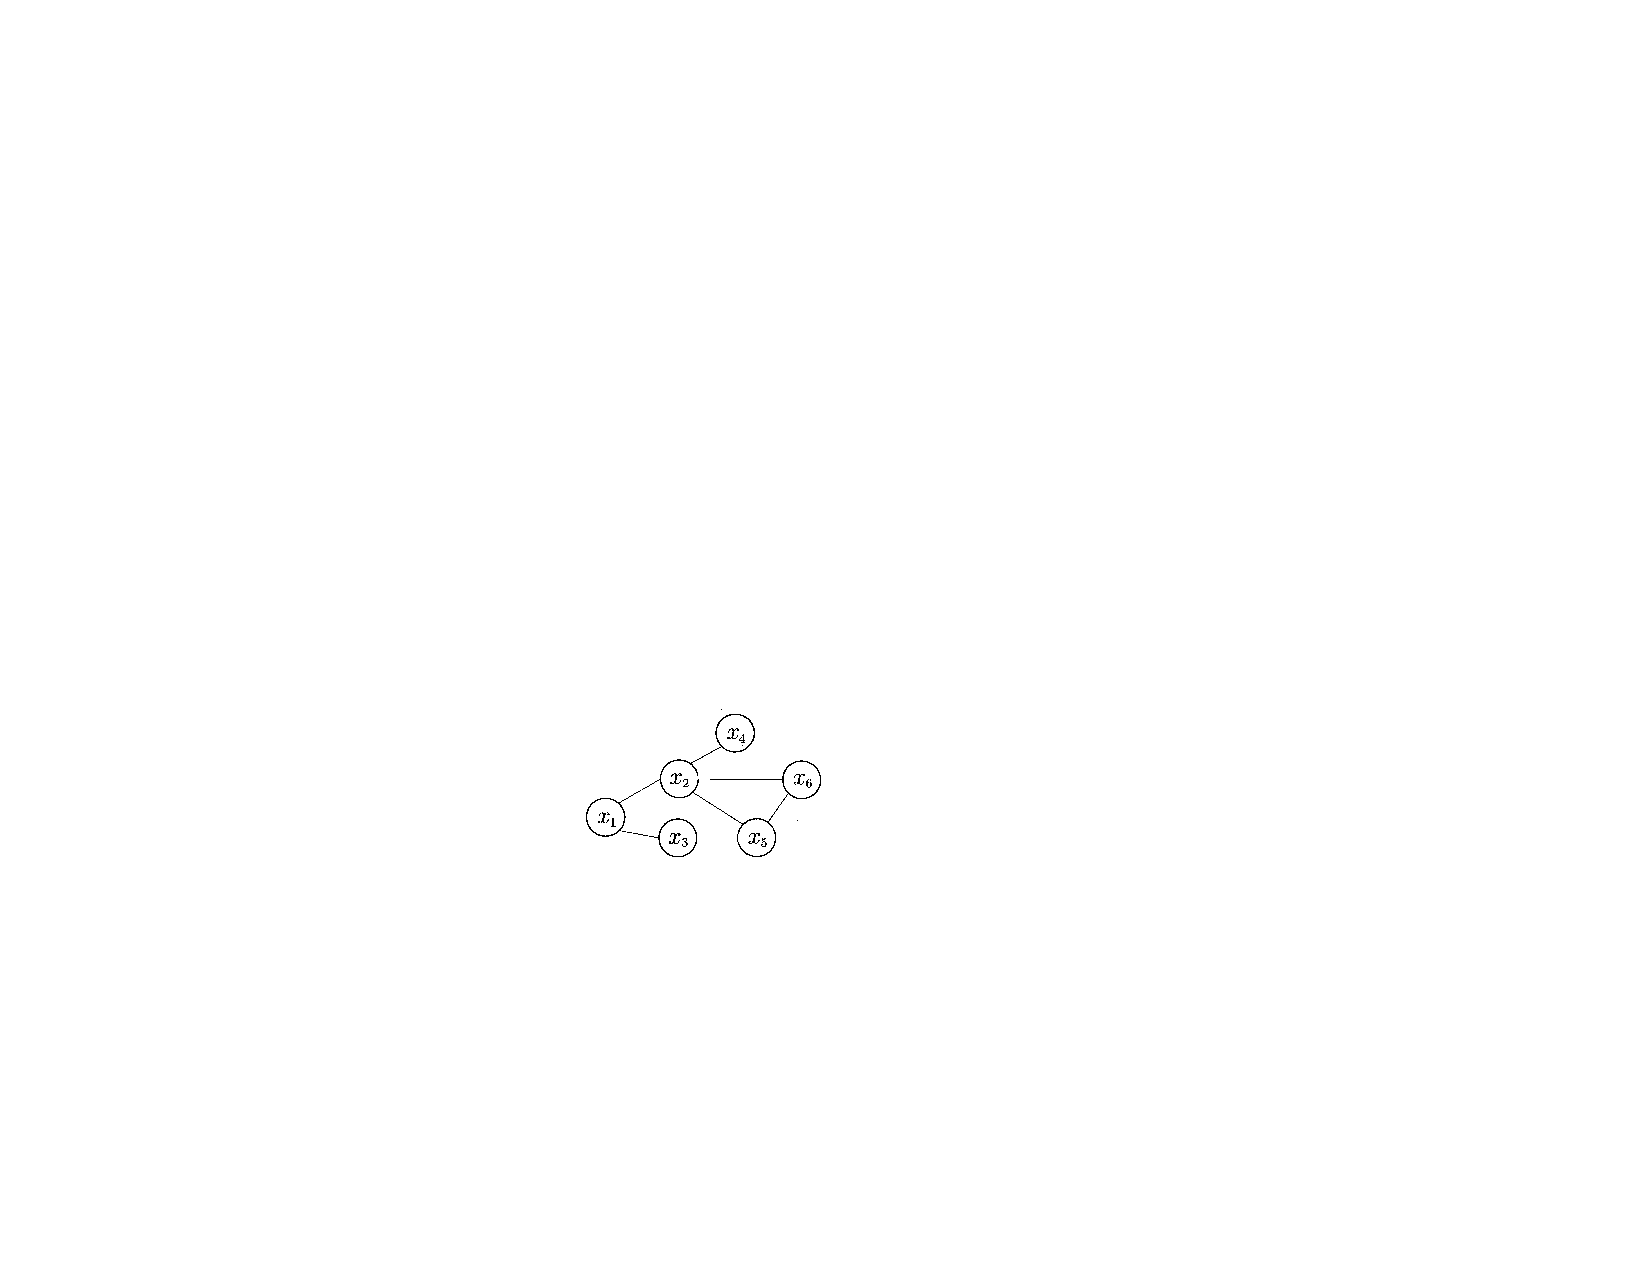
\includegraphics[width=0.7\textwidth]{figures//4.pdf}
\caption{马尔可夫随机场}
\label{default}
\end{center}
\end{figure}
\par 马尔可夫随机场具有两个重要的特性:
\begin{itemize}
\item 局部马尔可夫性:给定某变量的邻接变量,则该变量条件独立与其他变量。
\item 成对马尔可夫性:给定所有其他变量,两个非接邻变量条件独立。
\end{itemize}
\subsection{图结构数据的建模方法}
Hanjun Dai\cite{dai2016discriminative}等人用马尔可夫随机场对图结构数据进行了建模。首先定义一个图结构数据$\chi$,其结点集合为$\mathit{V}=\{1,...,V\}$,边集合为$\xi$。对图结点中的每一个结点$V_i$,都有一个对应的特征向量$X_i$。这里的特征向量$X$为我们能够观测到的性质,相应的,对每一个特征向量$X_i$,我们定义一个额外的隐变量$H_i$,这样我们就将图结构的数据转换为了一个马尔可夫随机场,并且能够得到该随机场的联合概率分布:
\begin{equation*}
p(\{H_i\}, \{X_i\}) \propto \prod_{i\in V} \Phi(H_i, X_i)\prod_{(i, j)\in \xi} \Psi(H_i, H_j)
\end{equation*}
其中$\Phi$为$H_i$到$X_i$的观测函数,$\Psi$为$H_i$到$H_j$的状态转移函数。
\par 在这个模型中,在生成隐变量的过程中,不仅将图上的每个结点的特征作为输入,还考虑到了图的结构,将新生成的隐变量的结点按图结构连接起来,从而实现了既保留了图的数据又保留了图的结构。下图展示了建模的过程:
\begin{figure}[htbp]
\begin{center}

\includegraphics[width=0.8\textwidth]{figures//1.pdf}
\caption{图数据隐变量建模}
\label{default}
\end{center}
\end{figure}
\subsection{图结构数据模型的求解}
直接求解以上的马尔可夫随机场是十分复杂的,我们需要对图结构中所有结点的相互关系进行考虑求解,即:
\begin{equation*}
p(H_i|{x_i}) = \int_{\mathcal{H}^{V-1}} p(H_i, \{h_j\}| \{x_j\}\prod_{j\in V\i})dh_i
\end{equation*}
对上式的直接求解是十分困难的,现在主要的方法是运用平均场推断和信念传播网络求解估计值,本文采用了Hanjun Dai\cite{dai2016discriminative}提出的平均场推断的算法。
\par 平均场推断算法尝试用一个独立的密度成分$q_i(h_i)$来近似估计$p(H_i|{x_i})$,即$p(H_i|{x_i})=\prod_{i\in V} q_i(h_i)$,其中$q_i(h_i)\ge 0$,在平均场中所有成分的概率和为1即$\int_\mathcal{H} q_i(h_i)dh_i=1$。求解平均场中密度成分需要最小化平均场中的自由能(Wainwright和Jordan\cite{wainwright2008graphical}),即求解以下的最优化方程:
\begin{equation*}
\min_{q_1, ..., q_d} \int_\mathcal{H}^d \prod_{i\in V}q_i(h_i)\log \frac{\prod_{i\in V}q_i(h_i)}{p(\{h_i\}|\{x_i\})}\prod_{i\in V}dh_i
\end{equation*}
要实现上式的最小化,需要满足以下的等式:
\begin{align*}
\log q_i(h_i) &= c_i + log( \Phi(h_i, x_i)) + \sum_{j\in \mathcal{N}(i)} \int_\mathcal{H}\log (\Psi(h_i, h_j) \Phi(h_j, x_j))dh_j\\
&={c_i}'+ log( \Phi(h_i, x_i)) + \sum_{j\in \mathcal{N}(i)} \int_\mathcal{H}\log (\Psi(h_i, h_j))dh_j
\end{align*}
可以得到:
$$c_i' = c_i + \sum_{j\in \mathcal{N}(i)} \int_\mathcal{H}\log \Psi(h_i, h_j)  $$
其中$\mathcal{N}(i)$为隐变量$H(i)$在图模型中的相邻结点,$c_i$为常数。从上式可以得知$q_i(h_i)$的值与$h_i, x_i, \{q_j\}_{j\in \mathcal{N}(i)}$有关,由此可以定于一个关于$q_i(h_i)$的等式:
\begin{equation*}
q_i(h_i) =  f(h_i, x_i,  \{q_j\}_{j\in \mathcal{N}(i)})
\end{equation*}
对于平均场中的每个组成结点$q_i$,我们可以得到其在希尔伯特空间的映射:
\begin{equation*}
\tilde{\mu}_i = \int_{\mathcal{H}} \phi(h_i)q_i(h_i)dh_i
\end{equation*}
已知$q_i(h_i) =  f(h_i, x_i,  \{q_j\}_{j\in \mathcal{N}(i)})$,我们可以得到:
\begin{equation*}
\tilde{\mu}_i = \boldsymbol{\tau} (x_i, \{\mu_j\}_{j\in \mathcal{N}(i)})
\end{equation*}
其中$\boldsymbol{\tau}$为$\tilde{\mu}_i$与$x_i, \{\mu_j\}_{j\in \mathcal{N}(i)}$的映射关系,这样不需要求解马尔可夫随机场中的$\Phi, \Psi$两个函数,就可以得到$\tilde{\mu}_i$的表示方法。对于$\boldsymbol{\tau}$函数的具体函数我们可以通过对训练数据的学习来估计。本文采用了神经网络的方法来估计该函数。
\section{分类模型的构建}
\subsection{神经网络}
神经网络是由具有适应性的简单单元组成的广泛并行互联的网络,它的组织能够模拟生物神经系统对真实世界物体所作出的交互反应\cite{kohonen1988introduction}。神经网络中最基本的成分是神经元模型,每个神经元与其他神经元互联,当它“兴奋”(接收到数据被激活)时,就会向其相邻的神经元发送数据,改变相邻神经元的值,当相邻神经元的值超过某一阈值时,该神经元就被激活,从而向其他神经元继续发送数据。
\par 1943年,McCullich 和Pitts\cite{mcculloch1943logical}将上述情形抽象为“M-P神经元模型“。在这个模型中,神经元接受来自n个其他神经元的信号,这些信号通过带权重的连接进行传递,神经元接受到的总输入通过激活函数处理神经元产生的输出。
\begin{figure}[htbp]
\begin{center}
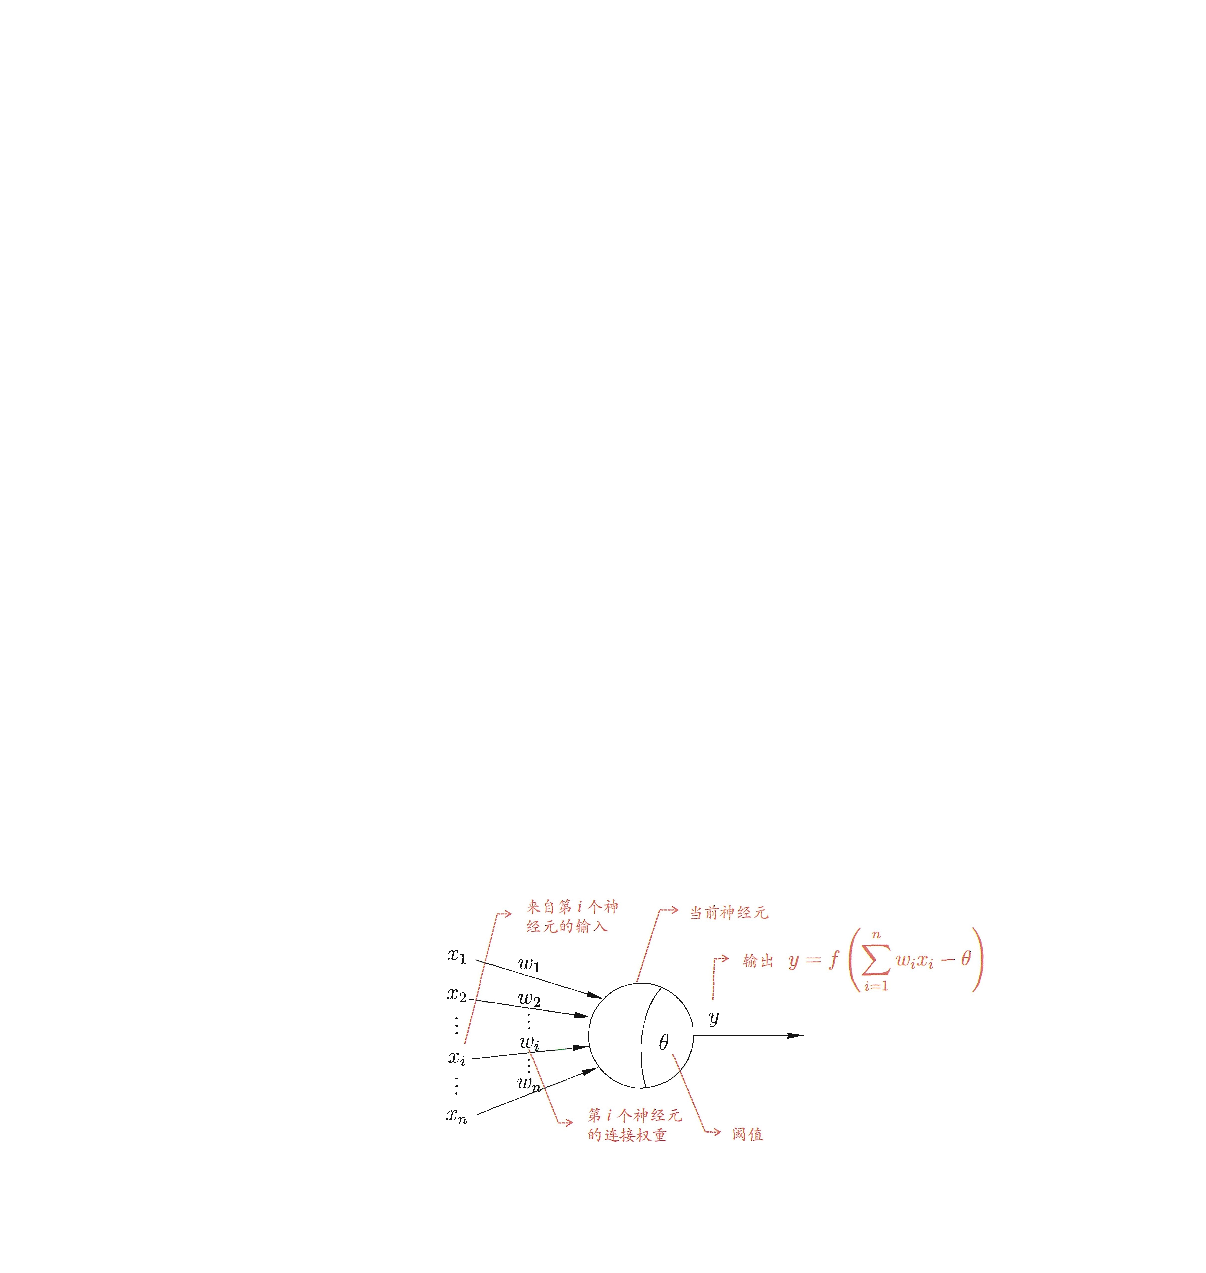
\includegraphics[width=0.75\textwidth]{figures//2.pdf}
\caption{M-P神经元模型}
\label{default}
\end{center}
\end{figure}
\par 理想中的激活函数为阶跃函数,当神经元激活时,输出1,抑制时输出0,然而在实际运用中,阶跃函数具有不连续,不光滑的性质,实际常用的函数有Sigmoid函数,可以把输入压缩到(0,1)的范围内,Relu函数可以丢弃值为负的神经元。
\begin{figure}[htbp]
\begin{center}
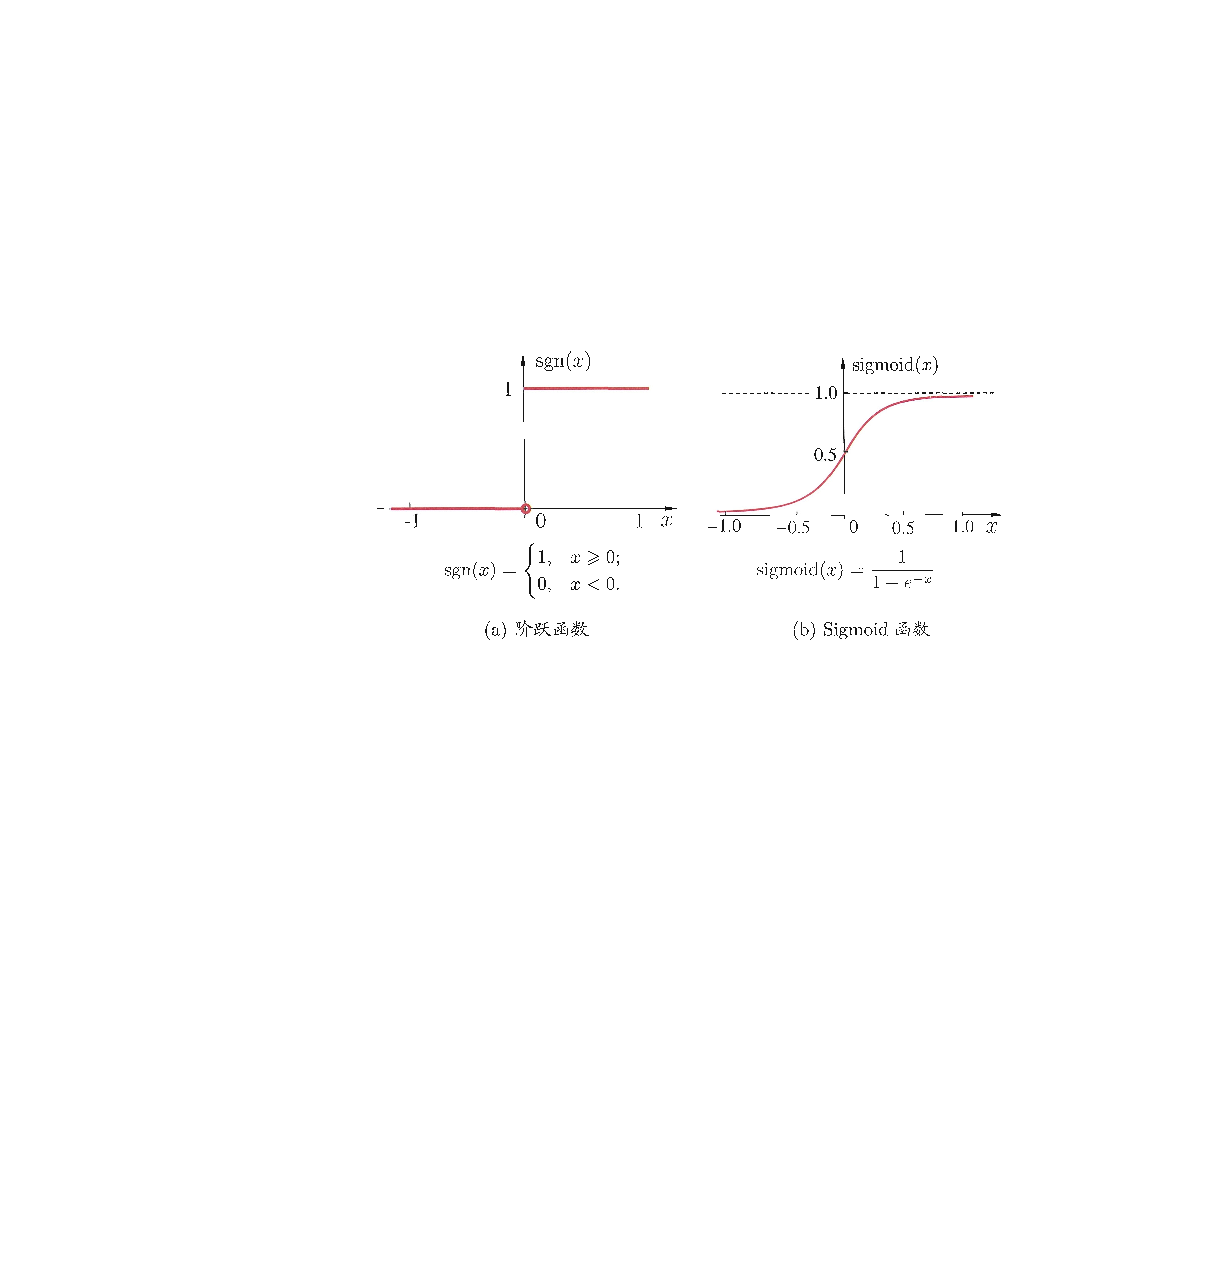
\includegraphics[width=0.8\textwidth]{figures//3.pdf}
\caption{常用激活函数}
\label{default}
\end{center}
\end{figure}
\par 从数学的角度来看,神经网络实际上是一个包含了许多参数的数学模型,可以看作是一个由$y_i = f(\sum_i w_ix_i-\theta_i)$这样的函数镶嵌叠加而成的复杂函数,当神经网络足够深时,这样的函数几乎逼近任意复杂度的连续函数,因此,可以用神经网络来代替难以求解的复杂函数,本文运用神经网络来逼近函数$\boldsymbol{\tau}$。
\subsection{图结构特征抽取模型构建}
上文中我们得到了$\tilde{\mu_i}$的表示函数:
\begin{equation*}
\tilde{\mu}_i = \boldsymbol{\tau} (x_i, \{\mu_j\}_{j\in \mathcal{N}(i)})
\end{equation*}
先用一个一层的神经网络对该函数进行逼近,则:
\begin{equation*}
\tilde{\mu}_i = \sigma(W_1x_i + W2\sum_{j\in \mathcal{N}(i)}\tilde{\mu}_j)
\end{equation*}
其中$\sigma$为relu的激活函数,$W_1, W_2$为网络的权重。假设得到的隐变量$tilde{\mu}_i$的维数为$d$,观测变量的维数为$p$,那么可以知道,$W_1$为一个$p*d$的权值矩阵,$W_2$为$d*d$的权值矩阵。为了更好的逼近函数$\boldsymbol{\tau}$,我们可以加深网络的深度$T$,进行多轮迭代更新$\tilde{\mu}_i$, 即:
\begin{equation*}
\tilde{\mu}_i^t = \sigma(W_1x_i + W2\sum_{j\in \mathcal{N}(i)}\tilde{\mu}_j^{t-1})
\end{equation*}
\begin{figure}[htbp]
\begin{center}
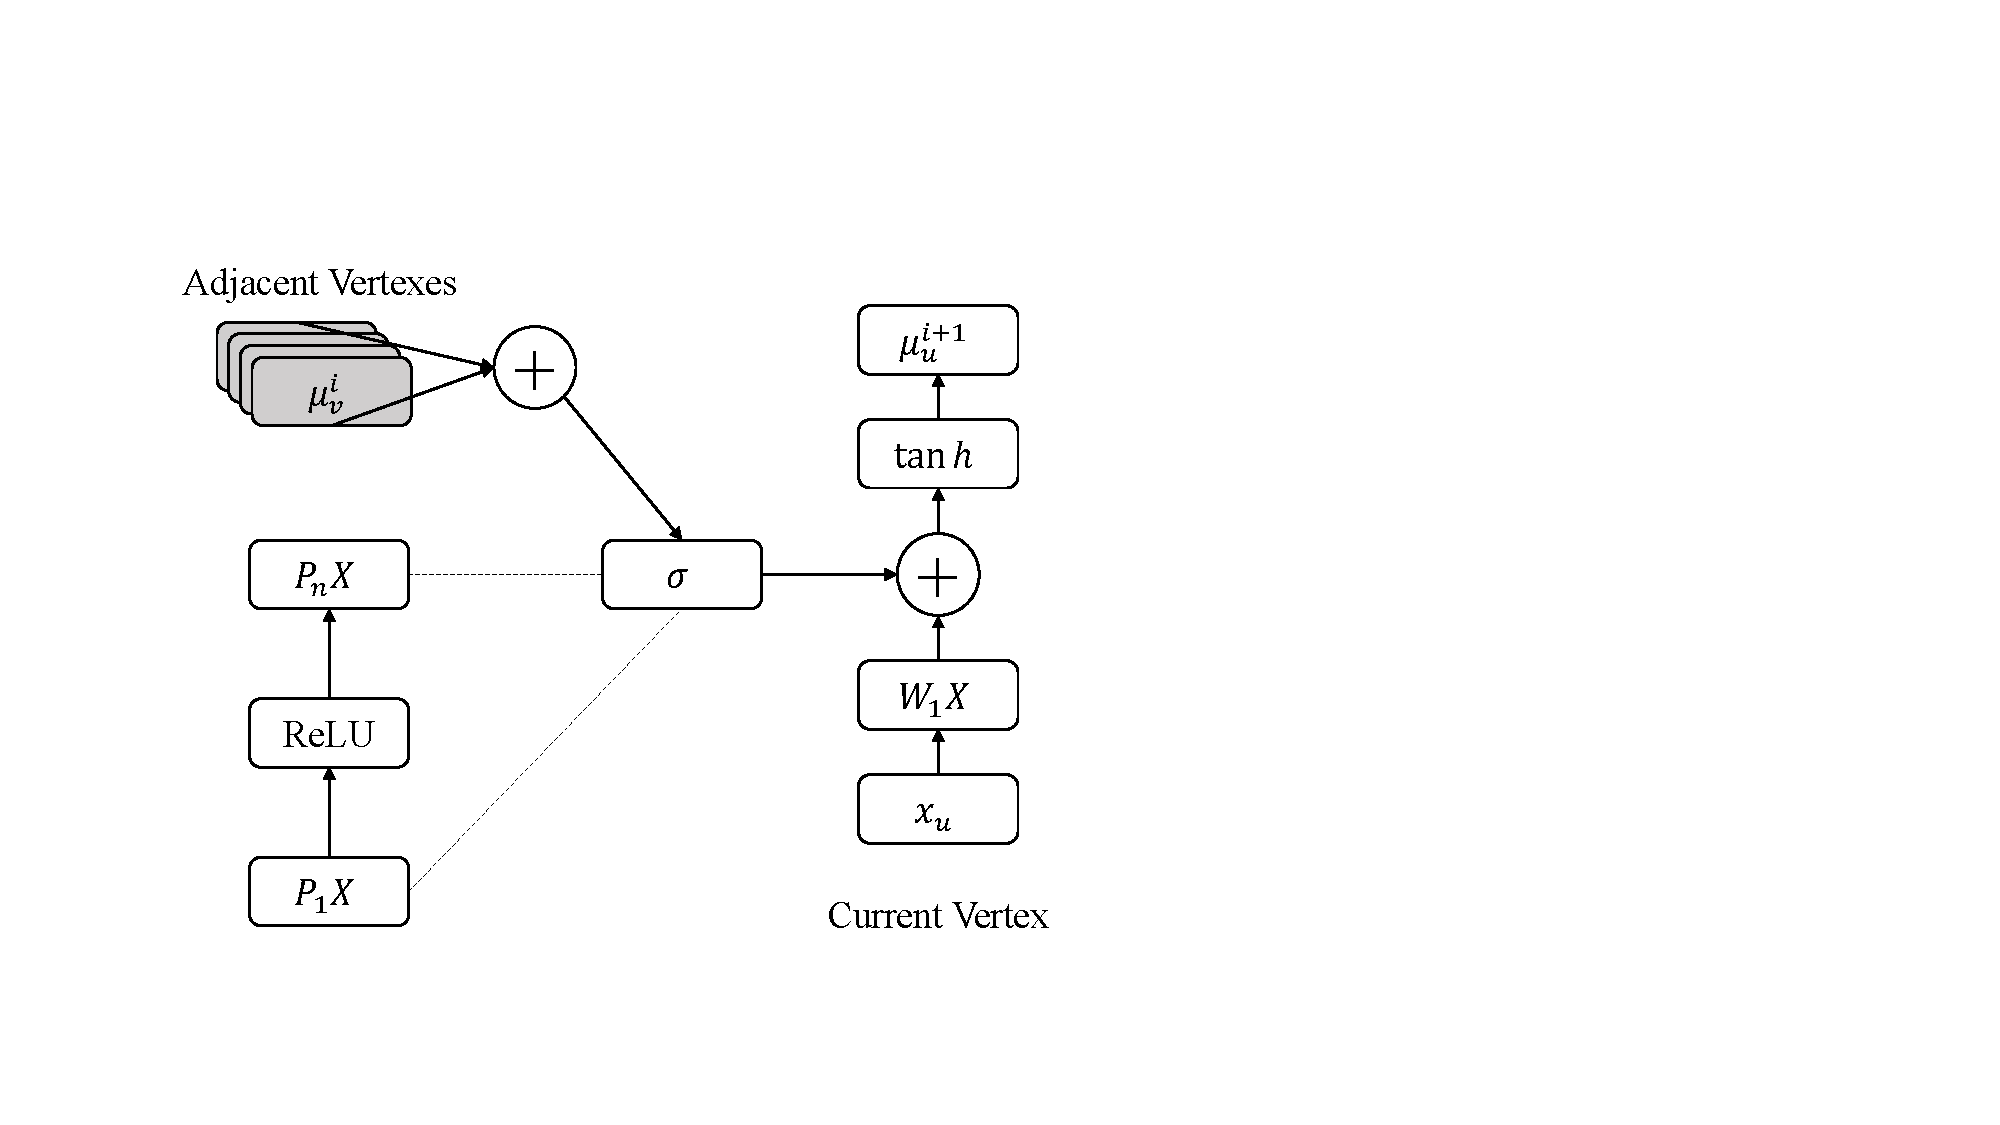
\includegraphics[width=0.7\textwidth]{figures//5.pdf}
\caption{图特征抽取模型图示}
\label{default}
\end{center}
\end{figure}
至此,对图结构数据中的每一个结点,都能够得到一个隐变量$\tilde{\mu}_i$,为了将图压缩为一个$n$维的向量$g$,我们可以将所有结点的隐变量求和:$g =\sum_{v\in V} \mu_v^{(T)}$。$g$中包含了图结构以及图结点的信息,对$g$进行分类相当于对图结构进行分类,并且$g$作为一个n维的向量,用神经网络继续分类将十分容易。得到$g$的具体算法过程为:
 \begin{algorithm}  
        \caption{Graph embedding algorithm}  
            \KwIn{$ACFG g = (V, \xi, x)$}
            \KwOut {$\phi(g)$}
            Initialize $\mu_v^{(0)} = \overline{0}$, for all $v \in V$\\
            \For {$t = 1 \KwTo T$}{
            	\ForEach{$v\in V$}{
			 $l_v = \sum_{u\in \mathcal{N}(v)}\mu_{u}^{(t-1)}$\\
			 $\mu_v^{(t)} = tanh(W_1*x_v+\sigma(W_2*l_v)$\\
			 }
			 }
            \Return {$\phi(g) = \sum_{v\in V} \mu_v^{(T)}$}
    \end{algorithm}  
\subsection{判别模型的构建}
明确了图数据压缩网络后,就可以通过训练数据来学习网络中的参数。为了判定某段代码能否被一个静态检测工具正确的检测,需要一些先验的数据集 $D={x_n, y_n}_{n=1}^N$,其中$x_n$为抽取出来的代码的控制流图,$y_n$为代码的标签,如果该代码能够被工具正确检测,$y_n=[1, 0]$,否则$y_n=[0, 1]$,这是一个二分类的问题。我们需要学习得到一个网络,使网络得到的值能够最大的拟合训练数据,即:
\begin{align*}
&\min \sum_{n=1}^{N} (y_n - P*\phi(g))\\
&=\min \sum_{n=1}^{N} y_n - P*(\sum_{i=1}^{V_n} \tilde{\mu}_i^n)
\end{align*}
为了更好的拟合数据集$D$,逼近真实函数,我们在图结构压缩网络上定义了一个两层的非全连接网络$P$, $P$在两层全连接网络的基础上随机丢弃了一些神经元,从而避免了全连接网络可能存在的过拟合问题,具体来说,$P$可以定义为:
\begin{equation*}
P(\phi(g)) = W_4*(relu(W_3*relu(\phi(g))))
\end{equation*}
其中$W_3$为$d*d$的权值矩阵,$W_4$为$d*2$的权值矩阵。这样就得到了一个完整的图结构数据分类网络,该网络有四个权值矩阵$W_1, W_2, W_3, W_4$,以代码的控制流图为输入,输出一个$1*2$的向量$[a, b]$。当输出$a>b$时,代表工具检测正确的可能性大于错误的可能;若$a<b$代表工具检测错误的可能性最大。我们用梯度下降的方法对网络的权值进行更新,当输出值$[a, b]$与训练集的标签$y_n$残差较小且趋于稳定时,我们就得到了一个较好的用于区分某段代码能否被工具正确检测的分类网络。
\begin{figure}[htbp]
\begin{center}
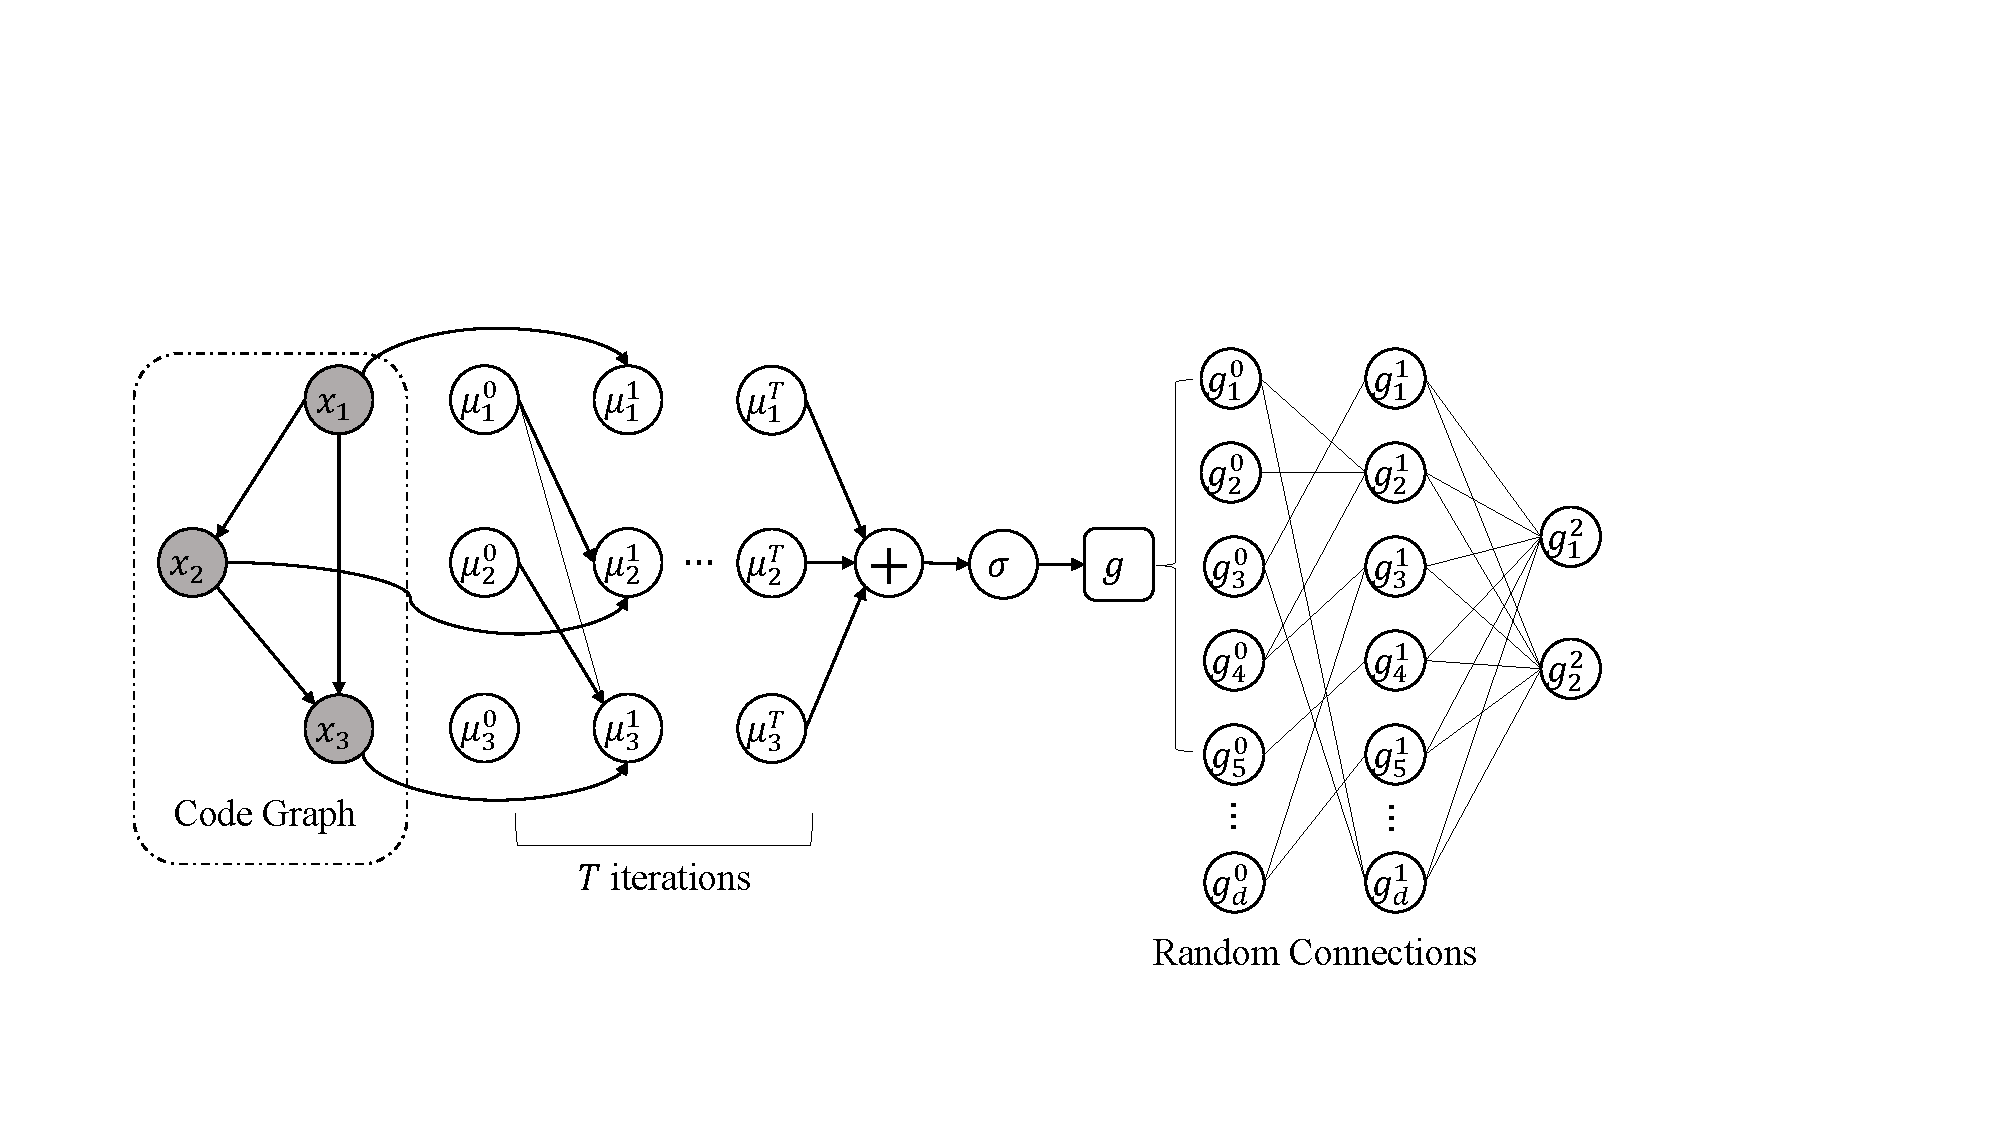
\includegraphics[width=0.95\textwidth]{figures//6.pdf}
\caption{完整分类模型图示}
\label{default}
\end{center}
\end{figure}
\par 基于此,对于四个静态代码分析工具,我们能训练出四个相应的分类器,这样,当检测一段未知的代码时,四个分类器能够分别得到四个工具检测这段代码的置信度$W = \{w_1, w_2, w_3, w_4\}$,同时我们能够得到四个工具对这段代码的检测结果$R = \{r_1, r_2, r_3, r_4\}$,这样综合两个结果,我们能够得到该代码是否存在空指针的置信度:
$$P = W^T*R = \sum_{i=1}^4 w_i*r_i$$
\par 设定好一个阈值$p$,当$P\le p$时,推断该代码段存在空指针;$P<p$,推断该代码不存在空指针。阈值$p$也可以通过学习得到,通过试错的方法逐渐更新$p$值,直到在训练集和测试集上得到最高的空指针检测准确率时,停止更新。
\section{本章小结}
本章介绍了代码分类神经网络模型的基本构造,阐述了图数据特征抽取模型的理论基础以及设计原理,介绍了分类模型神经网络的连接方式。最后阐明了神经网络的训练方法以及评判标准。